% !TEX program = xelatex
% ---------------------------------------------------------------------------
% 20-bit 40 MS/s SAR ADC 行为级验证模型 —— 专利与论文披露机制复现报告
% 引擎：XeLaTeX（Tectonic/XeTeX 0.17.0 亦可编译）
% 证据基线：tools/results/results.json
%   SHA256 = a1ccd92fcf46500460221a55c4e25270\allowbreak 93b45e6e272b7fb0503ee1fcd435ac70
% 版本基线：v7.0.7 (commit 8d00b80)
% ---------------------------------------------------------------------------
\documentclass[11pt,a4paper,fontset=fandol]{ctexart}
\usepackage[margin=2.2cm]{geometry}
\usepackage{amsmath,amssymb}
\usepackage{booktabs}
\usepackage{graphicx}
\usepackage{longtable}
\usepackage{array}
\usepackage{tabularx}
\usepackage{ragged2e}
\newcolumntype{P}[1]{>{\RaggedRight\arraybackslash}p{#1}}
\usepackage{enumitem}
\usepackage{xcolor}
\usepackage[colorlinks=true,linkcolor=blue!50!black,citecolor=blue!50!black,urlcolor=blue!50!black]{hyperref}
\usepackage{placeins}
\usepackage[htt]{hyphenat} % 允许 \texttt 内断字（长记录键）
\usepackage{needspace}

\definecolor{okgreen}{RGB}{0,120,80}
\definecolor{warnamber}{RGB}{176,102,0}
\definecolor{badred}{RGB}{176,32,32}

\newcommand{\GRADE}[1]{\textbf{#1}}
\newcommand{\rec}[1]{\texttt{#1}}
\newcommand{\uV}{\ensuremath{\,\mu\mathrm{V}}}
\newcommand{\nVrtHz}{\ensuremath{\,\mathrm{nV}\,\mathrm{Hz}^{-1/2}}}
\newcommand{\dBc}{\ensuremath{\,\mathrm{dBc}}}

\title{\heiti 20-bit 40\,MS/s SAR ADC 行为级验证模型\\[0.3em]
\Large 专利与论文披露机制的复现报告：证据、口径与边界}
\author{adi\_model 行为级验证模型（v7.0.7）}
\date{2026 年 9 月 11 日 \quad$\cdot$\quad 证据指纹
\texttt{a1ccd92f…35ac70}}

\begin{document}
\maketitle

\begin{abstract}
\noindent 本报告将 ISSCC~2024 9.8（文献 [00]/[00\_1]）及专利
[09]--[14] 所披露的关键技术，与 20-bit 40\,MS/s SAR ADC 行为级验证模型
（\texttt{adi\_model} v7.0.7）的仿真输出逐条对照，给出定量与定性复现
证据。复现口径与 \texttt{model\_scope.md}~\S1 一致：本模型校准对象是
\emph{已发表数值}（published figures），数值一致属于\textbf{兼容性/一致性
检查}，而非对实测硅片的预测；由 \GRADE{FITTED} 参数锚定的数字是锚点
构造的恒等式，不是独立预测，凡属此类均直接标注。全部数字取自参考输出
\texttt{tools/results/results.json}（SHA256
\texttt{a1ccd92fcf46…35ac70}，v7.0.5 全量复跑逐字节验证），每条证据
均给出记录键与参数来源等级。结果概览：\textbf{11 项定量对照}（按证据性质分级：\emph{推导/闭合类}、
\emph{读法假设下的条件自洽}、\emph{工程回归}，见 \S6 分级表）、
\textbf{13 项机制级对照}、\textbf{2 项原创扩展证据}（KTC 相消，
不归属 ADI）、以及\textbf{如实登记的 4 项未复现/负结果}。本报告不使用
``$N$ 项无自由参数复现''这类总括表述：不同条目支持不同强度的结论，
强度只能在分级表中逐条认领。全部证据以 27 行对照表加 \textbf{8 组图示对比}（披露机制自绘示意↔模型仿真数据）
呈现，并给出各条目的适用域边界与引用限制，防止把锚点恒等式或非因果实现的
实验数字误用作独立预测或设计预算。图示中的机制示意均为本报告自绘，
未复制任何第三方文档图像（引用合规）。
\end{abstract}

\clearpage
\tableofcontents
\newpage

% ===========================================================================
\section{引言：复现的对象与口径}
% ===========================================================================

\subsection{复现对象}

模型的架构研究对象是文献 [00] 披露的 20-bit 40\,MS/s、94.2\,dB~DR 精密
SAR 转换器：18-slice 电容池轮换、共享剩余放大器（RA）、采样态 dither、
9-bit 一级粗量化 + 精细 SAR 的两步结构、auto-zero 复位策略等。机制细节
对照专利 [09]（量化器分离与误差自愈）、[10]（dither 施加方法）、
[11]（DEM 线性化）等；[12]--[14] 的机制（交织跟踪、辅助输入、低功耗
参考）已随 v7.0.8 以\textbf{机制级独立模型}实现（M11--M13，各带专项
测试），但\textbf{尚未接入 pipeline 主链路}——N2 据此收窄为``主链路
集成未做''，接入属于会移动已发布数值的发版纪律事项（R1/R2 物理池
先行）。

\subsection{``复现''一词在本报告中的含义}

本模型是行为级验证模型，不是晶体管级复刻。因此本报告区分三种证据等级：

\begin{enumerate}[itemsep=1pt]
  \item \textbf{推导复现（DERIVED）}：由披露参数出发，经模型内部的独立
        方程推得，与披露数值吻合，\emph{无自由参数}。这是最强的复现
        等级，例如由披露的 20.5\,pF 采样电容推导 kT/C 噪声
        $\sigma = 20.10\uV$。
  \item \textbf{机制复现（定性/结构性）}：模型表现出与披露机制一致的
        \emph{结构性质或方向性行为}（如杂散位置、守恒律、边界两侧
        行为），数值不要求一一对应。
  \item \textbf{锚点恒等式（FITTED）}：数值一致是因为该参数本身由同一
        披露值反推锚定。这类一致只证明预算记账自洽，
        \textbf{不得}作为独立预测引用。
  \item \textbf{工程回归}：如同种子逐位一致（Q11），证明的是\emph{软件
        确定性与可重复执行}，不构成对任何物理机制的定量复现，单独归级。
\end{enumerate}

此外，个别条目为\textbf{条件性吻合}（扫描到特定物理参数时与披露值
吻合，如 INL 缺口）或\textbf{带限定的结果}（如洗牌 31.4\,dB 出自非因果
实现）。每张表的``一致性''列均按此口径措辞。

\subsection{证据链与可复现性}

\begin{itemize}[itemsep=1pt]
  \item 全部数字来自参考输出 \texttt{tools/results/results.json}，
        SHA256~$=$~\texttt{a1ccd92fcf46500460221a55c4e2527093b45e6e
        272b7fb0503ee1fcd435ac70}；该文件在 v7.0.5 发版时经全量复跑
        \textbf{逐字节比对}确认。
  \item 重跑入口为 console script：
        \texttt{adi-run-all -{}-results-dir <dir>}。
        \emph{不要}直接 \texttt{python tools/run\_all.py} 传
        \texttt{-{}-results-dir}——脚本只读环境变量，该 flag 会被静默
        忽略并把结果写回默认目录。
  \item 参数来源分级由 \texttt{provenance.py} 在运行时强制执行：
        \GRADE{DISCLOSED}（披露值直引）/ \GRADE{DERIVED}（无自由参数
        推导）/ \GRADE{FITTED}（锚定）/ \GRADE{ASSUMED}（假设）。
        本报告所有证据行均附等级标签。
  \item 工程状态：v7.0.7（commit \texttt{8d00b80}），门禁 ruff /
        format / mypy 全净，pytest \textbf{189 passed, 4 xfailed}，
        远端 CI 结论 success。
\end{itemize}

% ===========================================================================
\FloatBarrier
\section{定量复现结果（Q1--Q11）}
% ===========================================================================

\subsection{总表}

表~\ref{tab:quant} 给出披露值与模型值的逐条对照。``一致性''列的措辞
即证据等级；``证据记录''列为 \texttt{results.json} 中的记录键。

\begingroup\footnotesize\sloppy
\setlength{\tabcolsep}{4pt}
\begin{longtable}{@{}P{0.5cm}P{2.8cm}P{3.8cm}P{2.9cm}P{2.7cm}P{1.7cm}@{}}
\caption{定量复现：披露值 $\leftrightarrow$ 模型输出}\label{tab:quant}\\
\toprule
\textbf{\#} & \textbf{披露（出处）} & \textbf{模型输出} & \textbf{一致性判定} & \textbf{证据记录} & \textbf{等级}\\
\midrule
\endfirsthead
\multicolumn{6}{l}{\tablename~\thetable{}（续）}\\
\toprule
\textbf{\#} & \textbf{披露} & \textbf{模型输出} & \textbf{一致性判定} & \textbf{证据记录} & \textbf{等级}\\
\midrule
\endhead
\bottomrule
\endfoot
Q1 & NSD 8.8\nVrtHz{}、DR 94.6\,dB（[00\_1]） & NSD 8.93\nVrtHz{}、SNDR 93.55\,dB（20.5\,pF、无 KTC） & 数值吻合（$\approx$1.5\%）——\textbf{但 RA 噪声由 DR 目标反推锚定，属锚点恒等式，非独立预测} & \rec{s7\_dem\_off}、\rec{sweep} & FITTED\\
Q2 & 采样电容 20.5\,pF $\to$ kT/C（[00\_1]） & $\sigma=20.10\uV$（$\chi=2$ 差分）；kT/C 单独 DR~$=$~100.47\,dB（口径：20.5\,pF 为\emph{噪声等效电容}——分段网络折算后的值，非单边物理电容；公式正确不代表该值可代入任意节点） & 由披露电容\textbf{推导}，无自由参数 & \rec{validate}、\rec{derived} & DERIVED（口径限定）\\
Q3 & dither 量程 ``enhanced by 2b''（[00]） & \rec{units\_per\_lsb1}~$=$~4（一个一级粗步长含 4 个 DAC 单位步长，$\Delta_1{=}4\Delta_{\mathrm{DAC}}$）$\Rightarrow$ $b_1{=}7$ 读法下增强位数 $\log_2(512/128)=2.0$\,bit；一级总位 9.0\,bit；vra 摆动预测 0.1875\,V vs 实测 0.1736\,V（吸收率 92.6\%） & \textbf{条件自洽}（读法算术自洽，非唯一解证明，见正文） & \rec{validate}、\rec{dither\_quant}、\rec{derived} & 读法 ASSUMED\\
Q4 & 量化器/RDAC 匹配 ``$>$12b AC matching''（[00\_1] p.9） & 余量预算 9.6\,mV/300\,mV $\Rightarrow$ 等效匹配 \textbf{13.29\,bit}~$\geq$~12（推导链见正文；披露指标为 SADC$\to$RDAC \emph{采样响应}匹配，与静态电容失配不是同一指标） & 推导链需假设补全后自洽 & \rec{validate} & ASSUMED\,{+}\,DERIVED\\
Q5 & $G_0=32$（[00\_1] 图标注） & 电荷一致：$C_F = C_{\mathrm{active}}/G_0 = 640.625$\,fF，PASS & 推导一致 & \rec{validate} & DISCLOSED\\
Q6 & 后端不劣化 20b 目标（架构要求） & $\Delta_2/G_0 = 0.6\cdot\mathrm{LSB}_{20} \leq \mathrm{LSB}_{20}$ & 定量 & \rec{validate}、\rec{derived} & DERIVED\\
Q7 & SADC 粗码误差自愈窗口（[09]~\S1.3） & 预测窗口 4.6875\,mV；扫描（网格 1.17\,mV，\rec{window\_ok=true}）给出\textbf{边界区间} $[4.45,\,4.92]$\,mV：最后通过点 4.4531、首次失败点 4.9219（误差 10.9\uV、溢出 0.6\%）；7.03\,mV 处 302\uV & \textbf{机制定量复现}（配置条件值 $=$~ADC2 余量$/G_0$；修复域仅限粗码偏差） & \rec{pipeline.sadc\_window} & DERIVED\,{+}\,限定\\
Q8 & AZ 噪声代价 $-1.6$\,dB、ADC2 动态带宽 $+1.3$\,dB（[00\_1] p.34--35） & 整机折算预测 $-1.238$/$+0.923$\,dB vs 实测 $-1.233$/$+0.917$\,dB；叠加 $-0.223$ vs $-0.224$\,dB；\textbf{最大偏差 0.006\,dB} & 预算模型\textbf{内部一致}（功率线性）；与披露值的差额\textbf{归因待定}（参照系或预算口径可能不同），不硬凑 & \rec{autozero} & DISCLOSED（系数）/ 预算模型\\
Q9 & dither 三要素配对（[10]） & $\alpha$（配置）$=0.9923076923076923$ vs $\alpha$（掩码推导）$=0.9923076923076922$，差 $1.1\times10^{-16}$；离散码集 $[-2..2]$ SNDR 92.167\,dB $=$ 连续基准 92.167\,dB & \textbf{闭合到浮点舍入级} & \rec{dither\_closure} & DERIVED\\
Q10 & 电荷守恒（CDAC 物理底线） & 闭式解 vs 独立节点矩阵最大差 \textbf{$1.06\times10^{-25}$\,C}；主循环 vs 节点方程 $1.10\times10^{-25}$\,C（含信号$+$dither$+$DAC 电荷逐样本） & \textbf{闭合到 $10^{-25}$\,C（$\approx6.6\times10^{-7}$ 个基本电荷）}——连续电荷模型两条数值路径的浮点级一致性，非亚电子电路精度 & \rec{dither\_closure}、\rec{s12\_summary} & 结构性质\\
Q11 & 同种子可复现（工程要求） & 同芯片同控制：maxdiff~$=$~\textbf{0.0\,V}（逐位） & 精确 & \rec{s2} & 结构性质\\
\end{longtable}
\endgroup

\subsection{重点条目讨论}

\paragraph{Q1（NSD/DR）：锚点恒等式，不是预测。}
模型的 RA 噪声系数由 DR~94.6\,dB 目标\emph{反推}锚定，因此
NSD~8.93 与披露 8.8\nVrtHz{} 的吻合只说明噪声预算记账自洽
（参考输出无泄漏、无双重计数）。引用该数字时必须声明锚点性质。
独立的推导证据是 Q2：由披露电容 20.5\,pF 出发的 kT/C 项。

\paragraph{Q3（dither 增强 2\,bit）：两条披露联立的读法。}
[00] 披露 dither 量程``enhanced by 2b''。模型参数
\rec{units\_per\_lsb1}~$=$~4 的含义是\textbf{一个一级粗量化步长包含
四个 DAC 单位步长}（$\Delta_1=4\,\Delta_{\mathrm{DAC}}$）——它描述
的是粗级与细级步长的比例，\emph{不是}``dither 单位数 $=4\cdot
\mathrm{LSB}_1$''。在该配置下取一级细 SAR 位数 $b_1=7$，得量程扩展
$\log_2(512/128)=2.0$\,bit。注意结论的方向：这证明的是\textbf{$b_1=7$
这一读法与披露值算术上自洽}，$b_1=7$ 并非原文唯一读法（对比文档已标注
ASSUMED）；DAC 单位权重、粗级步长、整数/分数 dither 与模拟注入/数字
扣除各自的单位不能不经权重换算就视为同一物理量。交叉证据为 vra
（dither 吸收网络）摆动预测 0.1875\,V vs 实测 0.1736\,V，吸收率
92.6\%。0.067\,dB 的代价数字仅指当前衰减模型；``两种物理实现等代价''
还需列明比较时保持不变的电容、噪声、满量程与 dither 覆盖范围。

\begin{figure}[ht]\centering
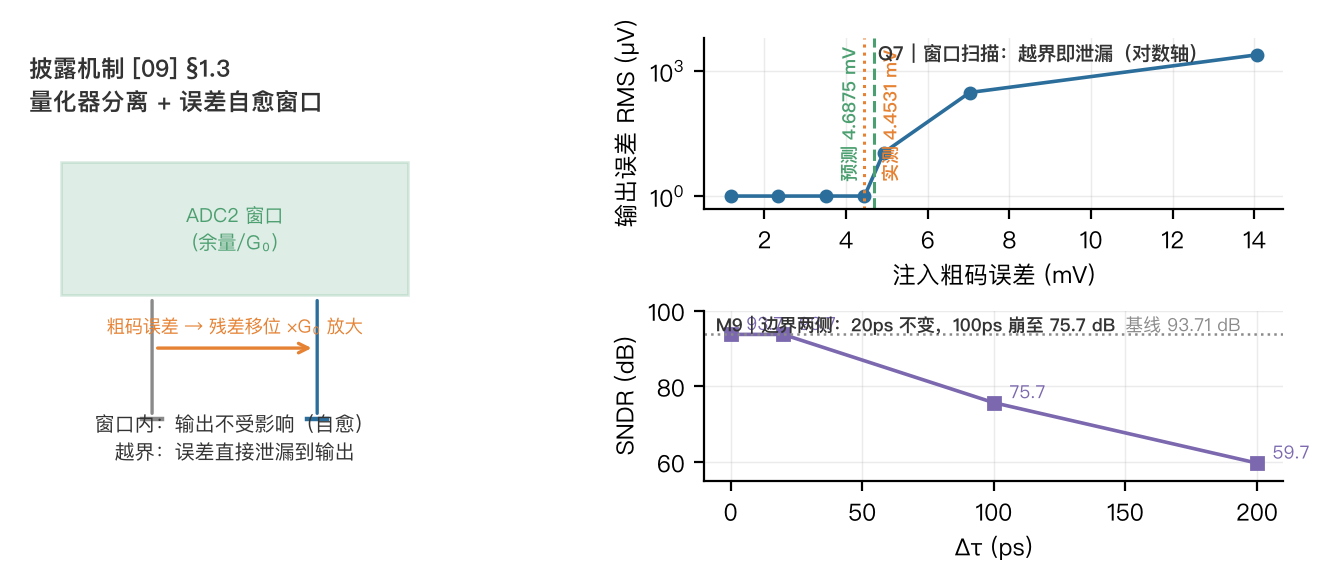
\includegraphics[width=\textwidth]{figs/fig3_sadc_window.png}
\caption{\textbf{SADC 误差自愈窗口（Q7/M9，[09]~\S1.3）}——左：披露机制示意
（自绘）：粗码误差将残差推出名义 bin，经 $G_0$ 放大后仍落在 ADC2 窗口内即被
吸收；右：模型三点式证据（\rec{pipeline.sadc\_window}、\rec{s9.coarse\_correction}）。
上图：注入粗码误差扫描（对数轴），预测窗口 4.6875\,mV（绿虚线，$=$~ADC2
余量$/G_0$）；橙点线为扫描边界区间 $[4.45,\,4.92]\,$mV（网格 1.17\,mV），
越界后误差从 \textasciitilde1\,µV 跳至 10.9\,µV~$\to$~302\,µV；下图：$\Delta\tau$ 扰动，20\,ps 时 SNDR 不变
（93.71\,dB），100\,ps 超窗崩至 75.7\,dB——边界两侧均被复现。}
\label{fig:f3}
\end{figure}

\paragraph{Q7（[09] 误差自愈窗口）：预测—实测—越界三点。}
[09]~\S1.3 披露粗量化误差不直接叠加到输出：残差被推离名义 bin，
只要放大后仍在 ADC2 窗口内即可被吸收。模型给出三点式证据：
预测窗口 4.6875\,mV（$=$~ADC2 余量$/G_0$，\GRADE{DERIVED}）、
扫描给出的\textbf{边界区间} $[4.45,\,4.92]\,$mV（网格 1.17\,mV：
最后通过点 4.4531，首次失败点 4.9219——误差 10.9\uV、溢出 0.6\%；
7.03\,mV 处 302\uV，超出即溢出）。注意两点边界：其一，4.6875\,mV 是
\textbf{配置条件值}（当前量程与增益配置下的可恢复余量），不是专利披露
的固定容差；其二，自愈的修复域\textbf{仅限粗码偏差}——真实采样误差、
DAC 权重误差与残差增益误差不在其修复域（若 $x_R$ 采错，重构恢复的是
采错的值）。窗口验收同时声明：扰动注入位置为粗码、ADC2 无溢出、
真实/名义 DAC 一致、增益校准开启。

\paragraph{Q8（AZ 预算）：内部一致与参照系差额分开陈述。}
预算模型按固定次序相乘（白噪声 $\times\,10^{1.6/20}$；闪烁噪声项
在模型中整体关闭——这是\textbf{模型理想化假设}，[00\_1] 披露的是整机
约 40\,Hz 的 1/f 拐角，\emph{不能}表述为``披露电路消除了全部闪烁
噪声''）。预测值与模型实测值最大偏差 0.006\,dB——这是\textbf{预算模型
内部一致性}，也是本条目的正面结论。预测值（$-1.238$/$+0.923$\,dB）与
披露值（$-1.6$/$+1.3$\,dB）的差额\textbf{尚不能确定归因}：披露未给
参照条件，可能由参照系或噪声预算口径不同造成，模型不硬凑。该条目属于``披露效果的预算模型''，不是 AZ
电路的相位级噪声模型。图~\ref{fig:f7} 给出三组预测↔实测对照。

\begin{figure}[ht]\centering
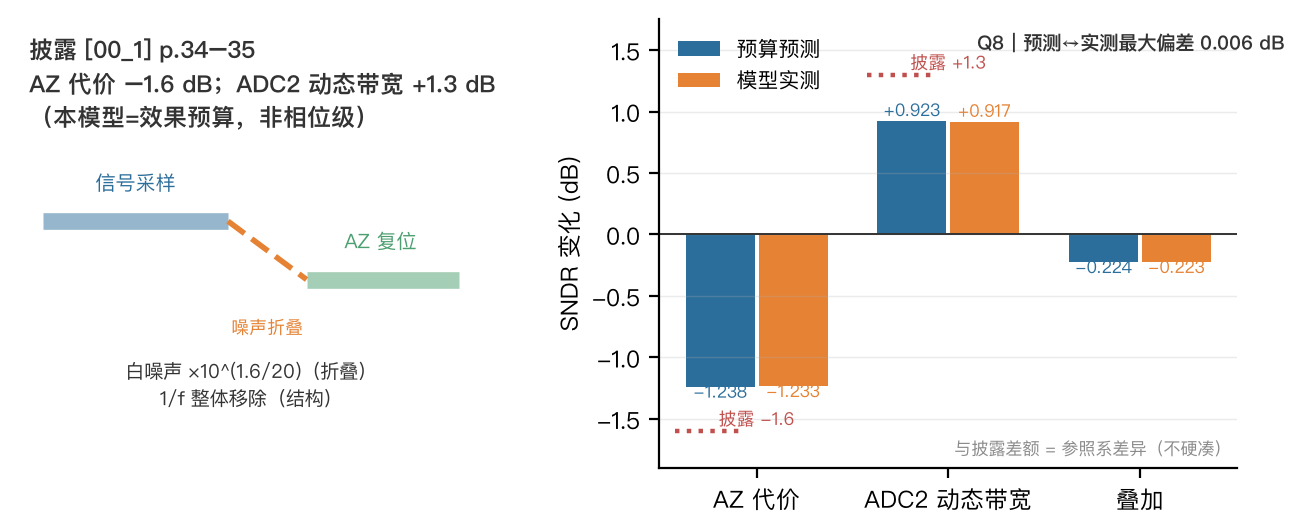
\includegraphics[width=\textwidth]{figs/fig7_autozero.png}
\caption{\textbf{Auto-zero 噪声预算（Q8，[00\_1] p.34--35）}——左：披露机制示意
（自绘）：AZ 复位相位引入白噪声折叠（$\times 10^{1.6/20}$）并移除 1/f；右：模型
预算预测与实测对照（\rec{autozero}）：三组（AZ 代价 / ADC2 动态带宽 / 叠加）
预测值与实测值最大偏差 \textbf{0.006\,dB}；红点线为披露值（$-1.6$/$+1.3$\,dB），
与预测值的差额\textbf{归因待定}（披露未给参照条件），不硬凑。}
\label{fig:f7}
\end{figure}

\paragraph{Q9/Q10（闭合检验）：复现的物理底线。}
dither 三要素（注入/改码/数字扣除）配对后，$\alpha$
衰减系数在配置与掩码独立推导两条路径上闭合到 $1.1\times10^{-16}$
（浮点舍入级）；分段 DAC 的闭式解与独立节点矩阵方程逐样本闭合到
$1.06\times10^{-25}$\,C——换算为 $\approx6.6\times10^{-7}$ 个
基本电荷。这两项的正确读法是：\textbf{连续电荷数学模型的两条独立数值
路径在当前测试条件下达到接近浮点舍入量级的一致}（实现一致性与局部
守恒检查）。它\emph{不}表明电路具有亚电子精度，也\emph{不}等同于
``其余全部数字都建立在物理守恒之上''——全局物理状态统一（R1/R2，
同一份电容真值同时驱动采样电荷/DAC 权重/增益/噪声）仍是开放里程碑
（\S7）。

% ===========================================================================
\FloatBarrier
\section{机制级复现结果（M1--M13）}
% ===========================================================================

\subsection{总表}

\begingroup\footnotesize\sloppy
\setlength{\tabcolsep}{4pt}
\begin{longtable}{@{}p{0.7cm}p{4.6cm}p{6.2cm}p{3.4cm}@{}}
\caption{机制级复现：披露机制 $\leftrightarrow$ 模型观察}\label{tab:mech}\\
\toprule
\textbf{\#} & \textbf{披露机制（出处）} & \textbf{模型观察} & \textbf{证据记录}\\
\midrule
\endfirsthead
\multicolumn{4}{l}{\tablename~\thetable{}（续）}\\
\toprule
\textbf{\#} & \textbf{披露机制} & \textbf{模型观察} & \textbf{证据记录}\\
\midrule
\endhead
\bottomrule
\endfoot
M1 & 交织杂散位置 $f_S/2\pm f_{\mathrm{IN}}$（[00]，结构性） & 带宽失配 spread~$=$~0.3 时杂散出现在 $f_S/2-f_{\mathrm{IN}}$，$-1.06\dBc$；spread~$=$~0 时该位置为噪声底 $-70.27\dBc$ & \rec{pipeline.interleave}\\
M2 & spare/洗牌打散交织杂散（[00]） & 固定组 $-1.06\dBc$ $\to$ 洗牌 $-32.46\dBc$（\textbf{31.40\,dB}）。{\bfseries 限定：}非因果洗牌实现（作用于误差系数）的结果，\textbf{不作为物理架构收益}；物理池接入主路径前不得用于匹配预算 & \rec{pipeline.interleave}\\
M3 & INL 2.2\,LSB（[00] 实测） & 动态误差三件套全开：确定性峰值 INL 6.70\,LSB（默认参数）；Ron 码调制扫描到 $\rho=0.035$ 时 \textbf{2.06\,LSB~$\approx$~论文 2.2\,LSB}（条件性吻合：解释 30$\times$ 缺口的是机制结构，不是把失配 $\sigma$ 硬调大） & \rec{s13}（\rec{rho\_max\_for\_2p2LSB}）\\
M4 & 参考建立 $\to$ 抛物线 INL（经典 bow） & 单开参考建立：INL$_{\max}$ 3.46$\to$4.39\,LSB，SNDR 几乎不变（低频失真被\emph{正弦拟合}吸收：去失调、去基波幅相；THD/SFDR 仍统计谐波）——符合``码相关、静态失配不可解释''的披露定位 & \rec{s13}\\
M5 & DEM 等权置换名义守恒（[11]） & \rec{nominal\_conservation.ok~$=$~true}：任意 state 下选中单位数 $=$ 逻辑码（\rec{k\_per\_code} 逐码核验） & \rec{s3}\\
M6 & DEM 消不掉桥接 $C_C$ 锯齿（[11] 边界预测） & DEM 开/关对 $C_C$ 比例误差锯齿的差 $\leq 5\%$（结构性质验证，非调参） & \rec{s12\_summary}\\
M7 & 交织映射的单位简并 $\to$ 参数辨识受限（[11] 跨 slice 动机） & 固定交织映射 $\mathrm{rank}(U)=\mathbf{127/512}$、DEM 轮转 313、随机置换 512（满秩）；整数码校准改善 fixed 0.8$\times$（恶化）/ dem\_rotate 15.5$\times$ / permute 6.8$\times$——满秩 $\neq$ 校准效果最好（条件数与噪声放大参与决定） & \rec{s14.maps}、\rec{s14.calibration}、\rec{s11\_summary}\\
M8 & dither 两种物理实现的代价（[10] Fig.6/19） & 输入注入 vs 采样态注入：等代价对比下采样态不占输入量程（溢出 0 vs 3.7\%）、代价 $=-20\log_{10}(\alpha)$（0.067\,dB @ $\alpha=0.9923$） & \rec{s9.dither\_impl}、\rec{dither\_closure}\\
M9 & SADC 误差自动修正边界（[09]~\S1.3） & $\Delta\tau=20$\,ps：粗码 2.3\% 变化、残差移 46.875\,mV（$=1\cdot\Delta_1$），SNDR 不变（93.71\,dB）；$\Delta\tau=100$\,ps 超窗：SNDR 崩至 75.7\,dB、溢出 3.4\%——\textbf{边界两侧都被复现} & \rec{s9.coarse\_correction}\\
M10 & 失配预算 $\to$ 校准必要性（架构论证） & SNDR~$\geq$~93\,dB 需 $\sigma\leq 300$\,ppm（均值口径 200\,ppm 极限）；PDK 估算 1117\,ppm，缺口 3.7$\times$；MC 16 片：93.30--93.72\,dB（$\sigma=100$\,ppm，FITTED） & \rec{budget}、\rec{mc}、\rec{derived}\\
M11 & [12] 交织跟踪相位电荷核算 & $v_{\mathrm{hold}}[i]=x[i{-}1]$ 逐拍恒等式（最近另一颗结果，仅差 1 个复合周期）；慢信号 kickback 电荷比 reset $<0.2$；带宽 $\propto$ 电荷、噪声 $\propto \sqrt{\cdot}$；近 Nyquist 区间如实复现 & 模块测试（v7.0.8 新增，不在 results.json 指纹内）\\
M12 & [13] 辅助输入建立标度律 & $R_f$ 上限放大 $(C_f{+}C_{pg})/C_f$ 倍；最低要求带宽与驱动噪声同比例降；gate\_boost 使 $r_{on}$ 码调制结构性归零 & 同上\\
M13 & [14] 低功耗参考阈值逼零回路（A06 机制层） & 整定 \textbf{6 个转换周期}（披露``5 or 6''）；外部补电荷随周期衰减 $>2$ 个量级；稳态粗判决 mV 级误差在 $\Delta_1/2$ 自愈窗内、末位试 $<1$\,nV（$>$20b 等效） & 同上\\
\end{longtable}
\endgroup

\subsection{重点条目讨论}

\begin{figure}[ht]\centering
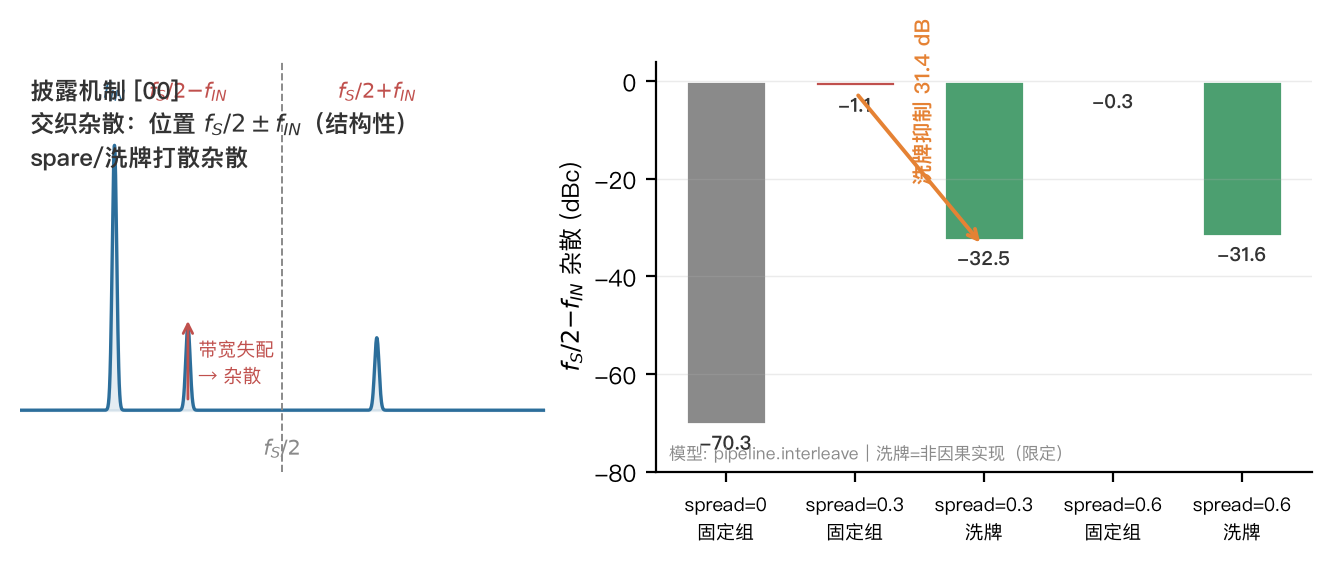
\includegraphics[width=\textwidth]{figs/fig1_interleave.png}
\caption{\textbf{交织杂散（M1/M2，[00]）}——左：披露机制示意（自绘）：带宽失配在
$f_S/2\pm f_{IN}$ 产生结构性杂散，spare/洗牌将其打散；右：模型测量
（\rec{pipeline.interleave}）：spread~$=$~0 时该位置为噪声底 $-70.3\,\mathrm{dBc}$，
spread~$=$~0.3 固定组 $-1.06\,\mathrm{dBc}$，洗牌后 $-32.46\,\mathrm{dBc}$
（\textbf{31.4\,dB}，非因果实现限定，M2）。位置与方向均与披露一致。}
\label{fig:f1}
\end{figure}

\paragraph{M2（洗牌 31.4\,dB）：数字本身有效，但用途受限。}
该 31.40\,dB 杂散改善出自当前 \texttt{ShuffledScheduler} 的\emph{非因果}
洗牌实现（直接作用于误差系数序列）。它证明了``打散交织杂散''这一机制
方向成立（[00] 披露的动机复现），但在 \texttt{PhysicalSlicePool}
（因果版，\rec{conv[n]=acq[n-1]}）接入主路径并重新测量之前，
\textbf{该数字不得写入物理架构收益或匹配预算}。此限定为第六份外部
复核订正，已钉入对比文档。

\paragraph{M3（INL 缺口）：条件性吻合的解释价值。}
论文实测 INL~2.2\,LSB，模型默认参数下动态误差三件套给出 6.70\,LSB。
把 Ron 码调制系数 $\rho$ 扫描至 0.035 时，模型 INL~$=$~2.06\,LSB。
这\emph{不是}把失配调大去凑数，而是给出条件性解释：在
$\rho\approx0.035$ 的物理量级下，机制结构（码相关 $\tau$、参考建立
bow、串扰三角形 $A(k)$）能复现 INL 的\textbf{量级}。\textbf{形状
对比须谨慎}：图~\ref{fig:f2} 左为本模型采用的误差形状示意（自绘），
\emph{不是}原文实测曲线的复现——原文给出的是跨码域正负起伏的实测
INL；``最大 INL 接近 2.2\,LSB''不等于整条 INL 曲线已复现。引用时须
注明 $\rho$ 条件。右上为 $\rho$ 扫描（条件性吻合点标注），右下为
动态误差三件套的机制对照。

\begin{figure}[ht]\centering
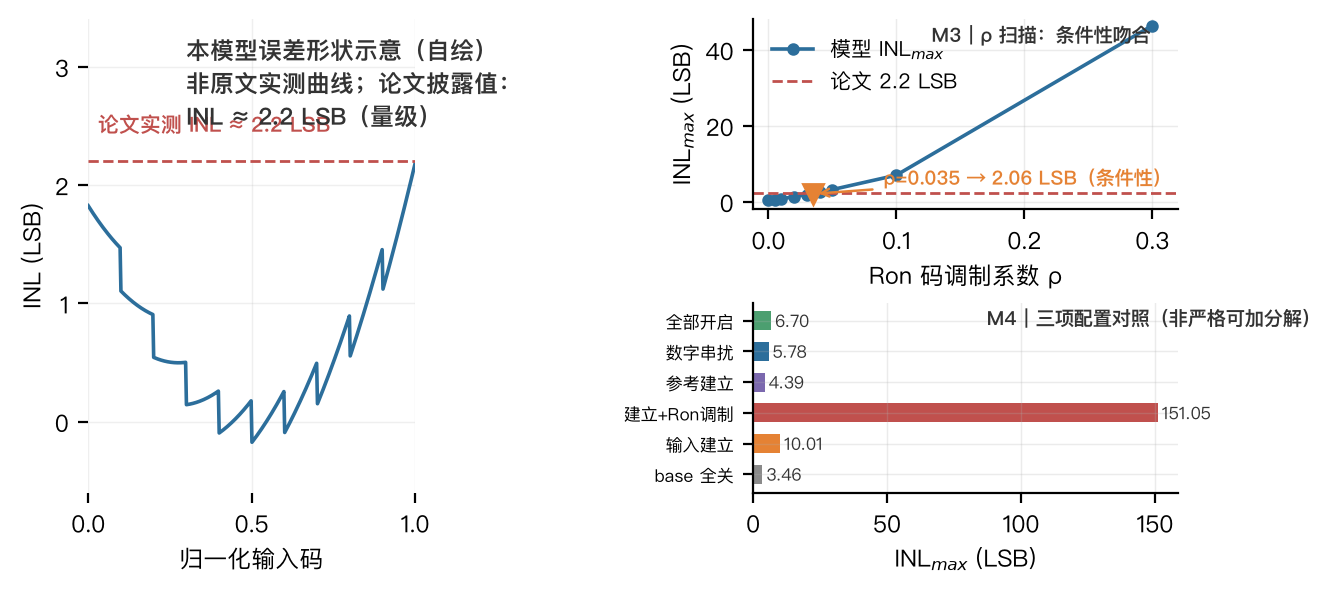
\includegraphics[width=\textwidth]{figs/fig2_inl.png}
\caption{\textbf{INL 形态与动态误差机制对照（M3/M4，[00]）}——左：\textbf{本模型
误差形状示意（自绘，非原文实测曲线）}，论文披露值 $\approx$2.2\,LSB；右上：模型
Ron 码调制扫描（\rec{s13.ron\_sweep}）：$\rho=0.035$ 时 INL$_{\max}=$~2.06\,LSB
$\approx$~论文 2.2\,LSB（橙三角标注，条件性吻合，取自 \rec{s13.rho\_max\_*}）；
右下：三件套机制对照（\rec{s13.rows}，单项实验配置与全开不同，不构成严格
可加分解）：``输入建立+Ron 调制''151\,LSB（主导项），全部开启 6.70\,LSB，
参考建立项 4.39\,LSB。}
\label{fig:f2}
\end{figure}

\paragraph{M9（[09] 边界机制）：两侧同时复现才算机制复现。}
[09] 的自愈机制只有同时展示``窗口内吸收''与``越界即崩''才是完整
复现。模型给出两侧：$\Delta\tau=20$\,ps（窗口内）SNDR 不变；
$\Delta\tau=100$\,ps（超窗）SNDR 从 93.71 崩至 75.7\,dB、溢出
3.4\%。边界位置与 Q7 的窗口预测一致（图~\ref{fig:f3} 右下）。

\paragraph{M5--M7（[11] DEM）：守恒成立、边界如实。}
DEM 等权置换的名义电荷守恒在任意 state 下逐码核验通过（M5，结构
性质）；桥接 $C_C$ 比例误差锯齿在 DEM 开/关之间的差 $\leq 5\%$，
即 DEM \emph{原理上}消不掉该项（M6）；固定交织映射的校准可观测性
固定交织映射 $\mathrm{rank}(U)=127/512$、DEM 轮转 313、随机置换
映射满秩 512（\rec{s14.maps}）。\textbf{口径限定}：秩不足限制的是
\emph{参数辨识}（512 个单位误差不能独立识别），不自动等于\emph{输出
误差不可校准}——只要待校正码的误差只依赖可观测参数组合，无需知道每颗
电容的独立误差；反之满秩也不保证校准好用（小奇异值/条件数/噪声放大：
本组数据中满秩 permute 改善 6.8$\times$，而 rank$=$313 的 dem\_rotate
改善 15.5$\times$）。三者共同构成 [11] 动机的复现：为什么需要跨
slice 的三维置换。见图~\ref{fig:f5}。

\begin{figure}[ht]\centering
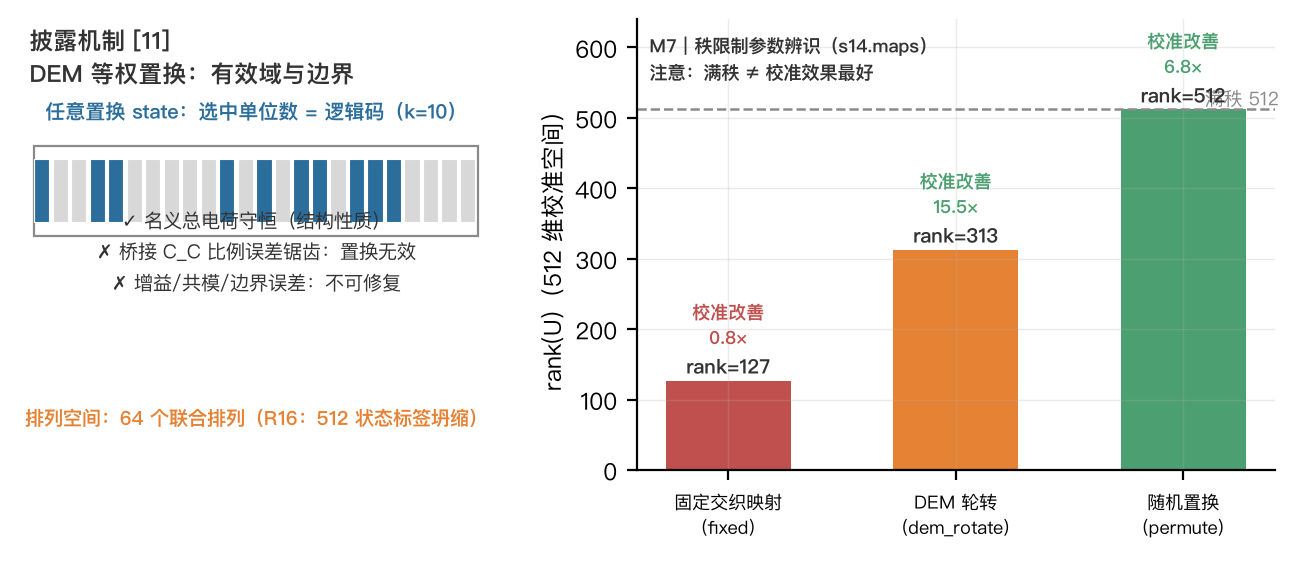
\includegraphics[width=\textwidth]{figs/fig5_dem.png}
\caption{\textbf{DEM 有效域与可观测性（M5/M6/M7，[11]）}——左：披露机制示意
（自绘）：等权置换保名义守恒，但 $C_C$ 锯齿/增益/共模/边界误差不在修复域，
联合排列空间为 64（R16，排列空间与矩阵秩是两个不同对象）；右：模型测量
（\rec{s14.maps}、\rec{s14.calibration}）：三种映射的 $\mathrm{rank}(U)$
（127/313/512）与整数码校准改善倍数（0.8$\times$/15.5$\times$/6.8$\times$）——
秩限制参数辨识，但满秩 $\neq$ 校准效果最好。}
\label{fig:f5}
\end{figure}

\paragraph{M8（[10] 两种 dither 实现）：等代价对比。}
输入注入（analog）与采样态注入（sampling）在等代价对比下：采样态
不占输入量程（溢出 0 vs 3.7\%）、代价 $=-20\log_{10}(\alpha)$
（0.067\,dB @ $\alpha=0.9923$），见图~\ref{fig:f4}。

\begin{figure}[ht]\centering
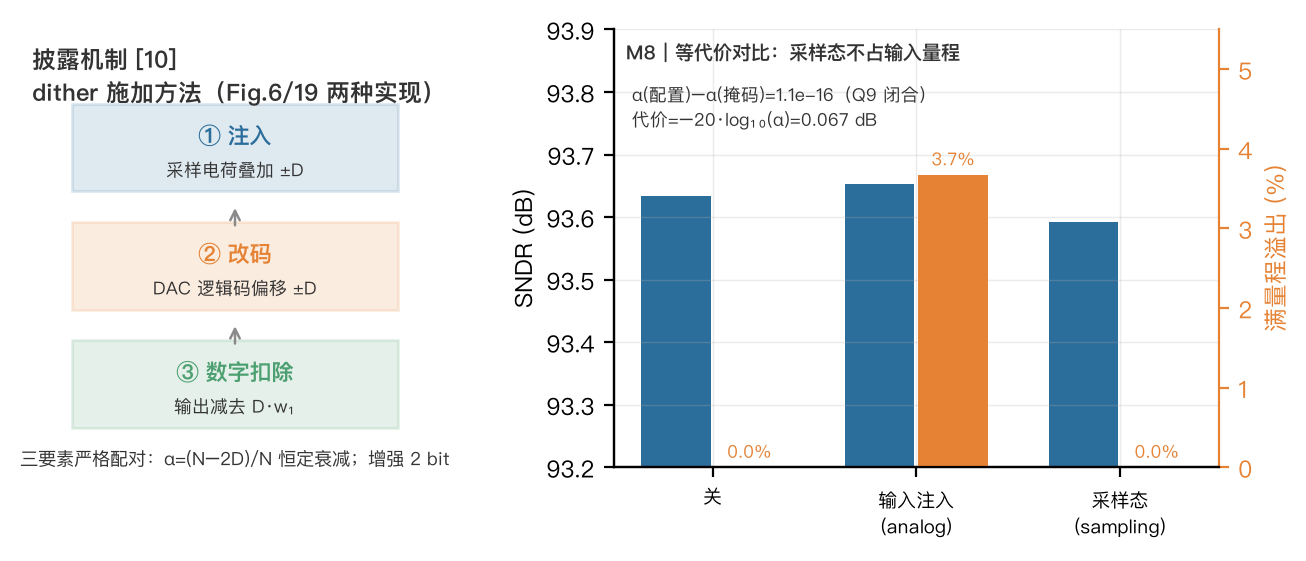
\includegraphics[width=\textwidth]{figs/fig4_dither.png}
\caption{\textbf{dither 施加方法（Q3/M8/Q9，[10]）}——左：披露机制示意（自绘）：
三要素（注入/改码/数字扣除）严格配对，$\alpha=(N-2D)/N$ 恒定衰减，量程增强
2\,bit；右：模型测量（\rec{s9.dither\_impl}）：三种模式的 SNDR 与满量程
溢出——采样态注入溢出 0\%（蓝 SNDR 柱 / 橙溢出柱），输入注入 3.7\%；
$\alpha$ 在配置与掩码两条独立推导路径上的闭合差为 $1.1\times10^{-16}$
（Q9，浮点舍入级）。}
\label{fig:f4}
\end{figure}

\paragraph{M10（失配预算）：校准动机的定量论证。}
\textbf{两个口径不得混写}：300\,ppm 是 [00\_1] 披露的匹配
\emph{目标}（文献常量），不是模型的达标点。模型自身的 $\sigma$ 扫描
（\rec{budget.rows}）给出：SNDR 均值 $\geq$~93\,dB 的达标上限
$\approx$~200\,ppm（93.13\,dB@200；92.56\,dB@300 已低于目标），最小值
口径 $\approx$~150\,ppm。PDK 估算 1117\,ppm 相对披露目标 3.7$\times$
缺口，等面积补偿需 $\approx$14$\times$ 电容——且面积改变会连带采样
噪声/输入负载/建立，\textbf{单纯扩面积不是等效替代}，由此得出校准是
更可行路径（``唯一出路''是过强表述）。映射链说明：披露指标是
SADC$\to$RDAC 的 AC matching（频率相关采样响应匹配），到``单位电容
失配 300\,ppm''再到``系统 SNDR''经过两级未在原文展开的映射，本模型
按此两级假设搭建（Q4）。MC 16 片为 $\sigma=100$\,ppm 配置组，
分布 93.30--93.72\,dB（FITTED）。

\begin{figure}[ht]\centering
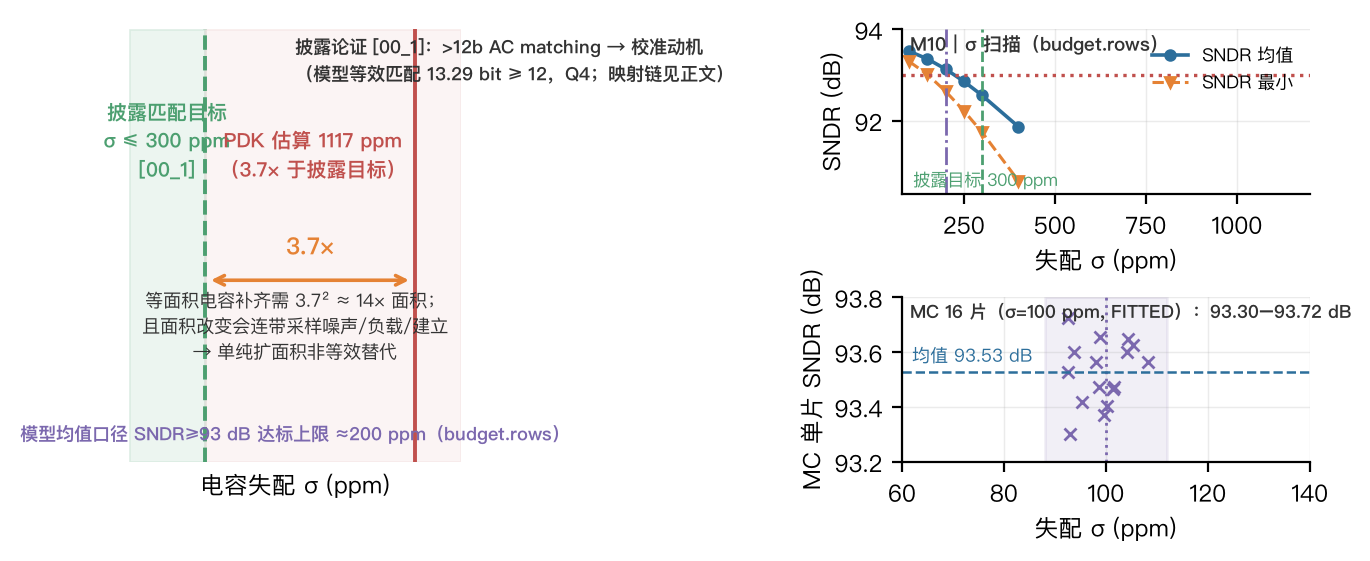
\includegraphics[width=\textwidth]{figs/fig8_budget.png}
\caption{\textbf{失配预算与校准动机（M10/Q4，[00\_1]）}——左：披露论证示意
（自绘）：\textbf{披露匹配目标} 300\,ppm vs PDK 估算 1117\,ppm（3.7$\times$），
等面积补偿需 $\approx$14$\times$ 电容且连带采样噪声/负载/建立——校准是
更可行路径；右：模型测量（\rec{budget.rows}）：$\sigma$ 扫描的 SNDR
均值/最小值曲线与 93\,dB 目标线；紫点线为\textbf{模型均值口径达标上限}
$\approx$200\,ppm（与披露目标 300\,ppm 是两个口径）；下：MC 16 片
（$\sigma=100$\,ppm 配置组，横轴即该组失配），分布 93.30--93.72\,dB。}
\label{fig:f8}
\end{figure}

\paragraph{M11（[12] 交织跟踪）：跟踪相位电荷核算。}
[12]~US~10,707,889~B1 把交织 SAR 的 IDLE 相位从``复位到中点''改为
``跟踪''——用\textbf{另一颗 sub-ADC 的最近转换结果}更新本颗 DAC，使
采集开始时保持电压已在前一样本电平附近。模型
（\texttt{interleave\_tracking.py}）在确定性轮换下复现逐拍恒等式
$v_{\mathrm{hold}}[i]=x[i{-}1]$（最近另一颗结果，仅差 1 个复合周期）；
慢信号下 kickback 电荷比 reset \textbf{$<0.2$}，且滤波器带宽
$\propto$ 电荷、驱动器噪声 $\propto \sqrt{\cdot}$ 的标度律成立
（[12] 披露的驱动收益方向）。加权模式复现披露例（N=3，10/30/60\%）。
近 Nyquist 区间（reset 反而更优，[12] 背景段 $Q{=}2A$ 算术的均值版）
\textbf{如实复现}，不做选择性呈现。机制级证据：模块测试 14 项
（v7.0.8 新增，不在 \texttt{results.json} 锁定指纹内）；主链路集成
未做（N2）。

\paragraph{M12（[13] 辅助输入）：寄生电荷的辅助通路核算。}
[13]~US~10,541,702~B1 用\textbf{不经过输入 RC 滤波器的辅助开关}给
采样网络的寄生电容充电，从而允许更低带宽/功耗的前级。模型
（\texttt{aux\_input.py}）给出其核心标度律：辅助通路接管寄生电荷后，
$R_f$ 允许放大 $(C_f{+}C_{pg})/C_f$ 倍，最低要求滤波器带宽与驱动
噪声同比例下降（噪声 $\propto \sqrt{R_f}$ 方向）；gate\_boost 模式下
$r_{on}$ 的码调制\textbf{结构性归零}（$V_{GS}$ 与采样值解耦）。这些
是机制层的倍率关系，不是某具体元件尺寸；主链路无第二输入端口
（N2）。机制级证据：模块测试 15 项。

\paragraph{M13（[14] 低功耗参考）：A06 机制层的回答。}
[14]~US~10,826,519~B1 以慢速功放 + 常充电大电容保持内部参考，转换
前只需极少量外部补电荷；模型（\texttt{ref\_track.py}）以限流充电 +
一阶伺服 + S1 泄放的行为级电荷-阈值回路复现其结构：\textbf{整定
6 个转换周期}（披露``5 or 6''）；外部补电荷随周期衰减 $>2$ 个量级；
阈值不动点 $\theta^{*}=-r$（跟随滞后，非零但相对逼零）。对审计
A06 的回答落在机制层：粗判决位试的参考误差为 mV 级（$\Delta_1/2$
自愈窗内，结构上可容忍），末位试误差 $<1$\,nV（$>$20b 等效）——
``参考仅 ~15b 精度时 RA 起动、尾段才到 20b''的方案由此自洽。
回路增益 $g$、泄放系数等参数为 \textbf{[假设]}（量级一致是结构
结果，非拟合主张）；主链路参考路径仍为瞬时增益（N2）。

% ===========================================================================
\section{原创扩展的证据（X1--X2，不归属 ADI）}
% ===========================================================================

KTC 噪声相消分支（\texttt{ktc.py}）为本仓库作者的\textbf{原创研究
扩展}，[00] 与专利 [09]--[14] 均未披露（NOTICE 已声明）。其证据
列于此仅供完整性，不构成对 ADI 披露的复现。

\begin{figure}[ht]\centering
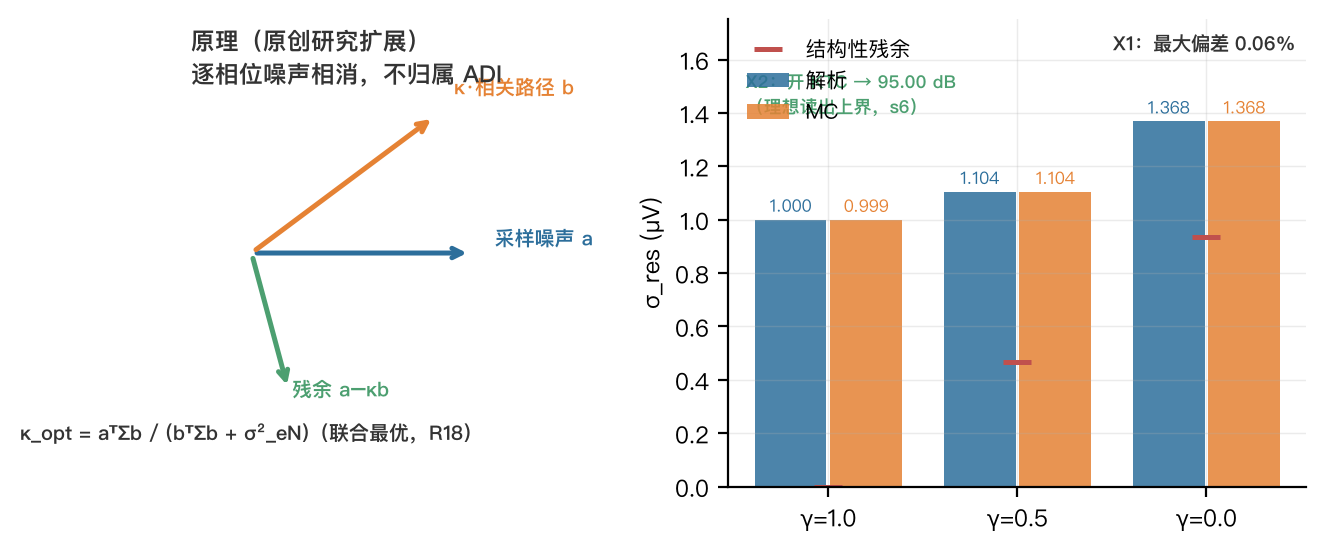
\includegraphics[width=\textwidth]{figs/fig6_ktc.png}
\caption{\textbf{KTC 逐相位噪声相消（X1/X2，原创研究扩展，不归属 ADI）}——左：
原理示意（自绘）：采样噪声矢量 $a$ 与相关路径 $\kappa b$ 相消后残余 $a-\kappa b$，
联合最优 $\kappa_{\mathrm{opt}}=a^{T}\Sigma b/(b^{T}\Sigma b+\sigma_{e_N}^{2})$（R18 修复）；
右：模型测量（\rec{noise\_transfer}）：$\gamma=1/0.5/0$ 三覆盖度下 MC（橙）
与解析（蓝）的 $\sigma_{\mathrm{res}}$ 对照——最大相对偏差 \textbf{0.06\%}，
红色横线为 $\gamma<1$ 时的结构性残余（$\gamma=0$：0.933\,µV）。X2：开 KTC
后 SNDR 93.70$\to$95.00\,dB（理想读出上界）。}
\label{fig:f6}
\end{figure}

\begin{itemize}[itemsep=2pt]
  \item \textbf{X1（逐相位噪声传递）}：噪声残余模型
        \[
          \sigma_{\mathrm{res}}^2
          = (a-\kappa b)^{\!T}\Sigma_Q\,(a-\kappa b)
            + \kappa^2\sigma_{e_N}^2 ,
          \qquad
          \kappa_{\mathrm{opt}}
          =\frac{a^{T}\Sigma_Q\,b}{b^{T}\Sigma_Q\,b+\sigma_{e_N}^{2}} .
        \]
        $\gamma=1/0.5/0$ 三覆盖度下，蒙特卡洛与解析 $\sigma_{\mathrm{res}}$
        最大相对偏差 \textbf{0.06\%}；$\gamma=1$ 残差 0.999\uV{}
        $\approx\kappa\sigma_{e_N}$；$\gamma=0$ 结构性残余 0.933\uV{}
        （占总采样噪声 4.4\%）；$\hat\kappa$ 回归与解析 $\kappa_{\mathrm{opt}}$
        吻合。其中含观测噪声的联合最优 $\kappa$ 为 v7.0.5 修复
        （R18，\rec{TestR18KappaOptimalWithObserverNoise} 钉子）。
  \item \textbf{X2（对 SNDR 的净收益）}：开 KTC 后 SNDR
        93.70$\to$95.00\,dB（\textbf{理想读出上界}：无量化器/编码/延迟
        模型）；观测噪声 20/50/100\uV{} 下仍 94.87--94.98\,dB。
        \textbf{节点口径}：$\sigma_{e_N}$ 为\emph{读取端等效}观测噪声
        （理想缓冲后的电压噪声源），观测过程假设不扰动原采样噪声状态、
        观测量无损进入数字域——这两条均未由实际读取电路建模支撑。解析
        与 MC 的一致验证的是\emph{所设统计模型的计算实现}，不自动证明
        观察电路可实现。引用时必须声明``理想读出上界''。
\end{itemize}

% ===========================================================================
\FloatBarrier
\section{未复现与负结果（N1--N4，如实登记）}
% ===========================================================================

\begin{longtable}{@{}p{0.7cm}p{5.2cm}p{9.2cm}@{}}
\caption{未复现项与负结果}\label{tab:neg}\\
\toprule
\textbf{\#} & \textbf{项} & \textbf{观察与口径}\\
\midrule
\endfirsthead
\toprule
\textbf{\#} & \textbf{项} & \textbf{观察与口径}\\
\midrule
\endhead
\bottomrule
\endfoot
N1 & dither 静态线性化收益 & \rec{s4.PASS\_失配下线性化有收益~$=$~false}：所测静态失配配置下 INL 1.598$\to$1.644\,LSB、$\sigma_e$ 2.90$\to$4.46\uV{}——dither 收益是\textbf{条件性}的（取决于误差结构），本配置无收益，与 scope 声明一致。\\
N2 & [12] 跟踪 / [13] 辅助输入 / [14] 参考电路 & 主链路零命中（\texttt{model\_scope.md}~\S4.12、A06），无从复现。\\
N3 & 论文三维 DEM 的定量收益 & 排列空间 \textbf{64~$\neq$~512}（R16：单个 \rec{sid} 同时驱动两个旋转，联合周期 $\mathrm{lcm}(64,8)=64$，512 个状态标签坍缩为 64 个联合排列）；本仓库 DEM 扫描\textbf{不得}引用为该机制的收益。\\
N4 & 实测硅片行为 & 一致性~$\neq$~预测（\texttt{model\_scope.md}~\S4.4）；DR~94.6\,dB 的再现是锚点恒等式（见 Q1）。\\
\end{longtable}

% ===========================================================================
\FloatBarrier
\section{复现等级汇总}
% ===========================================================================

按 \S1.2 的口径，全部证据分层如下：

\begin{table}[h]\centering\small
\begin{tabular}{@{}p{5.2cm}p{9.2cm}@{}}
\toprule
\textbf{等级} & \textbf{条目}\\
\midrule
推导/闭合类（DERIVED 或结构闭合） & Q2、Q5、Q6、Q7、Q9、Q10、M5\\
定量但锚定（FITTED 恒等式） & Q1——引用时\textbf{必须}声明锚点性质\\
预算模型一致性 & Q8（结构+系数对齐，非电路相位模型）\\
工程回归（软件确定性） & Q11（同种子逐位一致 $=$ 可重复执行，非物理复现）\\
读法假设下的条件自洽 & Q3（$b_1{=}7$）、Q4（推导链需假设补全）\\
机制/结构（定性或条件性） & M1--M13（M11--M13 为 v7.0.8 新增的专利 [12]--[14] 机制模型；M3 条件性；M2 带限定；M4 机制对照非严格分解）\\
条件性吻合 & M3（$\rho=0.035\to$2.06 vs 2.2\,LSB）\\
带限定 & M2（31.4\,dB，非因果实现）、X2（理想读出上界）\\
原创扩展 & X1、X2（不归属 ADI）\\
未复现/负结果 & N1--N4\\
\bottomrule
\end{tabular}
\end{table}

% ===========================================================================
\FloatBarrier
\section{与文献和专利的对应边界}
% ===========================================================================

复现证据必须与``实现到什么程度''一起阅读。表~\ref{tab:pat} 为
[09]--[14] 的逐专利对齐状态（对齐 / 机制对齐但口径不同 / 机制级实现
但主链路未接入），与仓库对比文档
\texttt{engineering\_vs\_patents\_papers.md} 保持一致（该文档已经第六
份复核订正：[12] 编号修正为 US~10,707,889~B1；18-slice、共享 RA、AZ
等条目的状态已与实际执行路径对齐；[12]--[14] 状态随 v7.0.8 更新）。

\begin{table}[h]\centering\small
\begin{tabular}{@{}p{3.6cm}p{5.6cm}p{3.6cm}p{1.9cm}@{}}
\toprule
\textbf{专利} & \textbf{机制} & \textbf{本仓库实现} & \textbf{状态}\\
\midrule
{}[09] US 10,516,408 B2 & 量化器分离 + 误差自愈窗口 & flash 阈值 + searchsorted；窗口定量验收 & \textcolor{okgreen}{对齐}\\
{}[10] US 10,505,561 B2 & dither 施加方法（三要素） & 注入/改码/数字扣除严格配对 & \textcolor{okgreen}{对齐}\\
{}[11] US 10,511,316 B2 & DEM 线性化 & 等权置换名义守恒 & \textcolor{warnamber}{机制对齐，排列空间 64}\\
{}[12] US 10,707,889 B1 & 交织跟踪状态更新 & \texttt{interleave\_tracking.py}：$v_{\mathrm{hold}}[i]=x[i{-}1]$ 恒等式；kickback 电荷比 reset $<0.2$；近 Nyquist 区间如实复现 & \textcolor{warnamber}{机制级实现，主链路未接入}\\
{}[13] US 10,541,702 B1 & 辅助输入抵消输入电荷 & \texttt{aux\_input.py}：$R_f$ 上限放大 $(C_f{+}C_{pg})/C_f$ 倍、最低带宽/噪声同比例降 & \textcolor{warnamber}{机制级实现，主链路未接入}\\
{}[14] US 10,826,519 B1 & 低功耗参考 & \texttt{ref\_track.py}：整定 6 个转换周期（披露``5 or 6''）；粗判决 mV 级容差、末位试 $>$20b 等效 & \textcolor{warnamber}{机制级实现，主链路未接入}\\
\bottomrule
\end{tabular}
\caption{专利对应状态}\label{tab:pat}
\end{table}

主链路的两个已知开放点（第六份复核 E10 确立的下一里程碑）：
\begin{enumerate}[itemsep=1pt]
  \item \textbf{物理 slice 池未接入主路径}：主入口
        （\texttt{pipeline.py} 348--354 行）仍将常量 \rec{c\_sig} 复制
        成数组传入 \rec{gain\_vector}，使用内部 \texttt{SlicePool}；
        \texttt{PhysicalSlicePool} 已通过独立验证但未接线。表~\ref{tab:mech}
        的 M2 及 31.4\,dB 数字均受此限定。
  \item \textbf{统一物理状态}：同一份电容真值尚未同时驱动采样电荷、
        DAC 权重、残差增益与噪声（R1/R2，xfail 登记）。
\end{enumerate}

% ===========================================================================
\FloatBarrier
\section{结论}
% ===========================================================================

\begin{enumerate}[itemsep=2pt]
  \item \textbf{定量层面}：推导/闭合类证据（Q2/Q5/Q6/Q7/Q9/Q10 及
        M5）覆盖 kT/C、SADC 自愈窗口、三要素闭合与电荷守恒；闭合精度
        分别为浮点舍入级（$10^{-16}$）与 $10^{-25}$\,C（$\approx
        6.6\times10^{-7}$ 个基本电荷——两条数值路径的浮点级一致性，
        非亚电子电路精度）。dither 增强（Q3）与 AC matching（Q4）为
        读法假设下的条件自洽，同种子一致（Q11）为工程回归，三者
        \textbf{不与推导类合并计数}。
  \item \textbf{机制层面}（图~\ref{fig:f1}--\ref{fig:f8}）：交织杂散位置、spare 打散方向、DEM 守恒与
        其不可修复边界（$C_C$ 锯齿、秩限制参数辨识）、自愈窗口两侧行为、
        失配预算与校准动机等 10 项披露机制在模型中表现出一致的
        结构性质。
  \item \textbf{口径纪律}：NSD/DR 吻合是锚点恒等式（Q1）；31.4\,dB
        是非因果实现结果（M2）；INL 吻合是条件性的（M3）；KTC 收益
        是理想读出上界（X2）。四项均须按限定引用。
  \item \textbf{未复现}：[12]/[13]/[14] 的\textbf{主链路集成}（机制级
        模型 M11--M13 已随 v7.0.8 实现，接入待 R1/R2）；论文三维 DEM 的
        定量收益（排列空间 64$\neq$512）；实测硅片行为超出口径。
  \item 下一步交付目标（第六份复核 E10）：让实际转换的那组电容真正
        决定该样本的保存电荷、DAC 权重、残差增益与噪声——
        \emph{物理主链路里程碑}，而非更多解释性文档。
\end{enumerate}

% ===========================================================================
\clearpage
\FloatBarrier
\begin{thebibliography}{00}\small
% 可选参数 = 正文手写编号，保持仓库编号体系
\bibitem[{[00]}]{ref00} R.~Bodnar et al., ``A 9.3\,nV/$\sqrt{\mathrm{Hz}}$ 20-bit
  40\,MS/s 94.2\,dB DR Signal-Chain Friendly Precision SAR Converter,''
  in \emph{IEEE ISSCC Dig. Tech. Papers}, Session 9.8, pp.~182--183, 2024.
  DOI: 10.1109/ISSCC49657.2024.10454329.
\bibitem[{[00\_1]}]{ref00p} ISSCC 2024 Session 9.8 presentation slides（作者自备稿,
  页码引用以 PPT 页码标注）.
\bibitem[{[09]}]{ref09} US~10,516,408~B2, ``Analog to digital converter stage.''
\bibitem[{[10]}]{ref10} US~10,505,561~B2, ``Method of applying a dither, and
  analog to digital converter.''
\bibitem[{[11]}]{ref11} US~10,511,316~B2, ``Linearizing transfer characteristic by
  dynamic element matching.''
\bibitem[{[12]}]{ref12} US~10,707,889~B1, ``Interleaving method for analog to
  digital converters.''
\bibitem[{[13]}]{ref13} US~10,541,702~B1, ``Auxiliary input for ADC input charge.''
\bibitem[{[14]}]{ref14} US~10,826,519~B1, ``Low power reference for an
  analog-to-digital converter.''
\end{thebibliography}

\noindent\textbf{引用合规声明}：以上仅列出条目（作者、会议/专利号、
DOI）。第三方文献与专利原文不在本仓库分发，版权归原权利人所有；完整
条目清单见仓库 \texttt{NOTICE}。

% ===========================================================================
\FloatBarrier
\appendix
\section{重跑与验证方法}
% ===========================================================================

\begin{enumerate}[itemsep=1pt]
  \item 环境：Python $\geq$3.11（3.13 已验证），依赖见
        \texttt{pyproject.toml}；安装后获得 console script
        \texttt{adi-run-all}。
  \item 全量复跑：
        \texttt{adi-run-all -{}-results-dir <dir>}（\emph{勿}直接
        \texttt{python tools/run\_all.py -{}-results-dir}，会被静默
        忽略）。
  \item 比对：对参考输出做 SHA256 校验，应得
        \texttt{a1ccd92fcf46500460221a55c4e2527093b45e6e272b7fb0503
        ee1fcd435ac70}；本报告所有记录键均可由该 JSON 直接索引。
  \item 测试：\texttt{pytest}（189 passed, 4 xfailed）；沙箱环境如遇
        \texttt{tmp\_path} 的 EEXIST 现象，加
        \texttt{-{}-basetemp=/tmp/<dir>} 复跑。
\end{enumerate}

\needspace{16\baselineskip}
\section{版本、门禁与审计状态}

\begin{table}[h]\centering\small
\begin{tabular}{@{}p{4.2cm}p{9.6cm}@{}}
\toprule
版本 & v7.0.7（commit \texttt{8d00b80}，tag 同步）\\
门禁 & ruff / ruff-format / mypy 全净；pytest 189 passed, 4 xfailed\\
CI & GitHub Actions 远端结论 \textbf{success}（含 Python 版本矩阵）\\
参考输出 & \texttt{results.json} 未变（v7.0.4 起逐字节一致）\\
审计 & 六份外部复核已逐条裁定；本报告对应第六份复核后的
        \texttt{reproduction\_results.md}，裁定文档
        \texttt{review\_response\_2026-09-11a--e.md} 共五份在库\\
边界文档 & \texttt{model\_scope.md}（适用域）、
        \texttt{engineering\_vs\_patents\_papers.md}（逐模块对应）、
        \texttt{key\_technologies.md}（十项关键技术）\\
\bottomrule
\end{tabular}
\end{table}

\end{document}
